\chapter{Experimentação}

\section{Teste de variação de entrada}

Foram executados testes randômicos variando as entradas dos programas. 
As palavras passadas ao programa variam em seu tamanho de 10 a 25 
caracteres. O script de teste captura antes de cada execução o tempo em
que a execução foi iniciada. Ao final para a contagem de tempo e escreve
os resultados em um arquivo de estatísticas. O programa que contabiliza 
o tempo foi baseado na bibliteca {\it sys/time.h} do sistema operacional 
GNU/Linux.

Abaixo estão os tempos de execução real, de usuário e de sistema 
de cada algorítmo em função dos tamanhos de entradas fornecidos aos 
programas: 

\begin{figure}[H]
    \begin{center}
        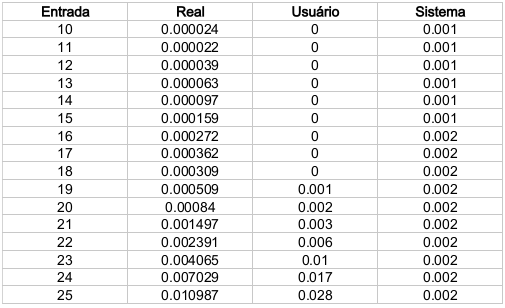
\includegraphics[width=0.8\textwidth,natwidth=610,natheight=642]{doc/brute-time-test.png}
        \caption{Tempo de execução - Força Bruta}
        \label{fig:brutetime}
    \end{center}
\end{figure}

\begin{figure}[H]
    \begin{center}
        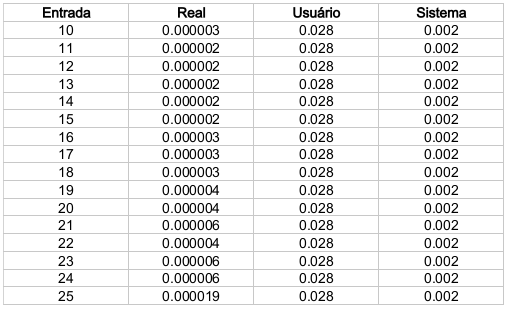
\includegraphics[width=0.8\textwidth,natwidth=610,natheight=642]{doc/dynamic-time-test.png}
        \caption{Tempo de execução - Programação Dinâmica}
        \label{fig:dynamictime}
    \end{center}
\end{figure}

\begin{figure}[H]
    \begin{center}
        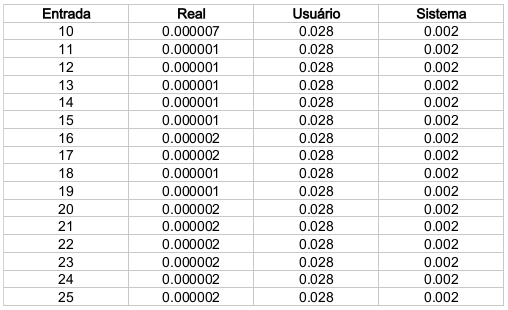
\includegraphics[width=0.8\textwidth,natwidth=610,natheight=642]{doc/greedy-time-test.png}
        \caption{Tempo de execução - Guloso}
        \label{fig:greedytime}
    \end{center}
\end{figure}

Como pode ser notado, para os tempos {\it reais}, com entradas de até 25 
caracteres de tamanho de palavra, o algorítmo \emph{guloso} se demonstrou
mais eficiente do que o \emph{dinâmico} e o \emph{força bruta}. No entanto
ele não é \emph{ótimo}. A seguir pode ser visto um comparativo entre as 
execuções dos algorítmos: 

\begin{figure}[H]
    \begin{center}
        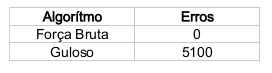
\includegraphics[width=0.8\textwidth,natwidth=610,natheight=642]{doc/errors.png}
        \caption{Erros em relação ao Dinâmico}
        \label{fig:errors}
    \end{center}
\end{figure}

Dado que o algorítmo utilizando o método da \emph{Programação Dinâmica}
é \emph{Ótimo} a figura \ref{fig:errors} apresenta um comparativo dos 
algorítmos \emph{Guloso} e \emph{Força Bruta} em relação ao 
\emph{Dinâmico}. Dado um arquivo de testes com 248832 entradas válidas 
para os algorítmos, foram executados os três programas e gerados os 
respectivos arquivos de resultados individuais. Em seguida foram 
comparados arquivos de resultado de cada algorítmo em relação ao 
resultado obtido pelo \emph{dinâmico}. Essa comparação mostra a 
disparidade e otimalidade das soluções propostas.

